%\textsc{}%\documentstyle[times,twocolumn,latex8]{article}
\documentclass[journal]{journal}
%\documentclass[times, 10pt,twocolumn,letterpaper]{article} 
\usepackage{cite}
%\usepackage{latex8}
\usepackage{times}
\usepackage[cmex10]{amsmath}
\usepackage[dvips,pdftex]{graphicx}
\usepackage{array}
%\usepackage{mdwmath}

%\usepackage{mdwtab}
%\usepackage[caption=false,font=footnotesize]{subfig}
\usepackage[tight,footnotesize]{subfigure}
%\usepackage[caption=false]{caption}
%\usepackage[font=footnotesize]{subfig}
%\usepackage{subfigure}
%\usepackage{helvet}
%\usepackage[bf]{caption}
%\renewcommand{\captionfont}{ \bf \small \fontfamily{phv}\selectfont }
%\renewcommand{\captionlabelfont}{\bf \small \fontfamily{phv}\selectfont }
%------------------------------------------------------------------------- 
% take the % away on next line to produce the final camera-ready version 
\pagestyle{empty}
%------------------------------------------------------------------------- 
\begin{document}
 \title{Comparing Arabic and Latin Handwritten Digits Recognition Problems}
\author{Sherif Abdelazeem
\\ shazeem@aucegypt.edu\\
Electronics Engineering Dept., The American University in Cairo\\
}
\maketitle
\thispagestyle{empty}
\begin{abstract}
A comparison between the performance of Latin and Arabic handwritten digits recognition problems is presented. The performance of ten different classifiers is tested on two similar Arabic and Latin handwritten digits databases. The analysis shows that Arabic handwritten digits recognition problem is easier than that of Latin digits. This is because the interclass difference in case of Latin digits is smaller than in Arabic digits and variances in writing Latin digits are larger. Consequently, weaker yet fast classifiers are expected to play more prominent role in Arabic handwritten digits recognition. %applications where classification speed is essential.
\end{abstract}
\begin{IEEEkeywords}
Handwritten recognition, Arabic recognition, Digits recognition 
\end{IEEEkeywords}
\section{Introduction}
Handwritten digit recognition problem can be seen as a sub-task of the more general Optical Character Recognition (OCR) problem. However, there are some applications (e.g., postal code and bank checks reading) that are restricted to recognizing digits but require very high accuracy  and speed. While recognition of handwritten Latin digits has been extensively investigated using various techniques \cite{benchmarking3}, too little work has been done on Arabic digits.

First, the issue of the names "Arabic digits" and "Latin digits" has to be resolved because naming conventions for different numeral systems may be confusing. Digits used in Europe and several other countries are sometimes  called "Arabic Numbers"; and digits used in the Arab world are sometimes called "Hindi Numbers". A different naming convention is used in this paper. Digits used in Europe will be referred to as "Latin Digits" and those used in the Arab world will be referred to as "Arabic Digits". It is worthwhile mentioning here that Arabic and Persian handwritten digits (digits used in Iran) are similar but not identical. Table \ref{tab:arabicandlatin} shows Arabic handwritten digits with different writing styles as well as their printed versions.

This paper compares the performances of different classification techniques on both  Arabic and Latin handwritten digit recognition problems. It is well known that there is no universally powerful or universally weak classifier \cite{PatternBook10}. The performance of a certain classification technique depends on how it matches the problem at hand. Realizing this, comprehensive comparative studies \cite{empiricalcomp11} compare the performances of classifiers on many different problems. However, if researchers doing such comparative studies do not have direct experience with the problems they use, they may not be able to give reasons.
\begin{table}
\begin{center}
\caption{Arabic Printed and Handwriten Digits.}
	\begin{tabular}{|l|l|l|l|l|l|l|l|l|l|l|}
	\hline
	Latin Equivalent & 0 & 1 & 2 & 3 & 4 & 5 & 6 & 7 & 8 & 9 \\ 
	\hline
	Printed & \includegraphics[scale=0.2]{images/0.JPG}  &  \includegraphics[scale=0.18] {images/1.JPG}   
	& \includegraphics[scale=0.2] {images/2.JPG} &  \includegraphics[scale=0.2] {images/3.JPG}  &\includegraphics[scale=0.2] {images/4.JPG}   & \includegraphics[scale=0.2] {images/5.JPG} 
&  \includegraphics[scale=0.2] {images/6.JPG}  & \includegraphics[scale=0.2] {images/7.JPG} 
	      & \includegraphics[scale=0.2] {images/8.JPG}   & \includegraphics[scale=0.2] {images/9.JPG}   \\ 
	\hline
	Typical Handwritten & \includegraphics[scale=0.2]{images/h0.JPG}  & \includegraphics[scale=0.3]{images/h1.JPG}   
	& \includegraphics[scale=0.2] {images/h2.JPG} &  \includegraphics[scale=0.2] {images/h3.JPG}  &\includegraphics[scale=0.2] {images/h4.JPG}   & \includegraphics[scale=0.2] {images/h5.JPG} 
&  \includegraphics[scale=0.2] {images/h6.JPG}  & \includegraphics[scale=0.2] {images/h7.JPG} 
	      & \includegraphics[scale=0.2] {images/h8.JPG}   & \includegraphics[scale=0.2] {images/h9.JPG}\\ 
	\hline
	Other Writing Style & -- & -- & -- & \includegraphics[scale=0.35] {images/h3_2.JPG}   & -- & -- & -- & -- & -- & -- \\ 
	\hline	
	\end{tabular}	
	\label{tab:arabicandlatin}
\end{center}
\end{table}
why a certain classification technique performs poorly on a certain problem while having a good performance on another. This paper attempts to understand the difference in performance of various classifiers when applied to the two different recognition problems of "Arabic" versus "Latin" handwritten digits. This should give researchers the chance to gain more insight into the natures of the two problems and, thus, be better able to do classifier-problem matching.

The remaining of the paper is organized as follows. Section \ref{sec:previouswork} is a survey of previous research on Arabic handwritten digits recognition problem that motivated this study. The classifiers and databases used in the comparison are described in Section \ref{sec:benchmark}. Section \ref{sec:compare} reports and analyzes the performances of the classification techniques on both the Latin digits and Arabic digits. Finally, the conclusion is in Section \ref{sec:conclusion}.
\section{Motivation} 
\label{sec:previouswork}
Little previous work has been done on Arabic handwritten digits recognition. Al-Omari et al.~\cite{indiannumerals14} proposed a system for recognizing Arabic digits from '1' to '9'. They used a scale-, translation-, rotation-invariant feature vector to train a probabilistic neural network (PNN). Their database was composed of 720 digits for training and 480 digits for testing written by 120 persons. They achieved 99.75\% accuracy. Said et al.~\cite{EnglishArabic15} used pixel values of the 16x20 size-normalized digit images as features. They fed those values to an Artificial Neural Network (ANN) with a dynamic number of hidden units. They used a training set of 2400 digits and a testing set of 200 digits written by 20 persons to achieve 94\% accuracy. It has to be noted that the results of different works can not be compared because the used databases do not have the same sizes or formats. Abdelazeem et al.~\cite{IjdarSherifPaper} did a comprehensive study on the problem of Arabic handwritten digit recognition problem. They introduced a large binary Arabic handwritten Digits dataBase(the ADBase ) and a modified gray level version of it (Modified ADBase or MADBase) and studied the performance of various classifiers/features combinations on the Arabic handwritten  digit recognition problem. The performances of well known feature extraction techniques followed by various classifiers have been analyzed in an approach similar to that followed by Liu et al.~\cite{benchmarking3} in their study of Latin handwritten digit recognition problem. Both ADBase and MADBase are available online for free at \textit{http://datacenter.aucegypt.edu/shazeem/}.

Comparing the results obtained in ~\cite{IjdarSherifPaper} for Arabic handwritten digits recognition problem with those in ~\cite{benchmarking3} for the Latin handwritten digit recognition problem reveals an interesting remark; and that is while the performance of a powerful classifier such as SVM is strong on both problems, the performance of less powerful classifiers such as linear or neural classifiers is better on the Arabic problem than on the Latin one. It is this observation that motivated the present comparative study in an attempt to understand the similarities/differences between the two problems. 
\section {The classification comparison}
\label{sec:benchmark}
The comparison between the Arabic and the Latin handwritten digit recognition problems is done by studying the performances of different classification techniques on Arabic as well as Latin handwritten digits on the raw pixel values of the digit images without any feature extraction. To make such a comparison valid, the used databases for Arabic and Latin digits should be of the same format. MNIST ~\cite{Gradient1} is the used Latin database while MADBase \cite{IjdarSherifPaper} is used as the Arabic database because it has the same size and format as MNIST ~\cite{Gradient1}. %Samples of 10 digits from MNIST and their corresponding digits from MADBase are shown in Figs. 1(a) and 1(b), respectively.
The present study uses 10 different classification techniques to compare between the MNIST and MADBase databases: LeNet 5 ~\cite{Gradient1}, Prazen window using RBF kernel ~\cite{PatternBook10}, artificial neural network (ANN), two different k-nearest neighborhood classifiers using k = 3 and k = 5, principle component analysis (PCA) with quadratic classifier, PCA with neural network classifier ~\cite{PatternBook10}, One versus All (OVA) linear classifiers, One versus One (OVO) linear classifiers, OVO SVM using linear kernel and finally OVO SVM using RPF kernel.
Each of those 10 classifiers is fed directly with gray-scale pixel values of digit images without feature extraction step. Some of the classifiers have parameters which need to be specified (e.g., the number of hidden units of ANN). Such parameters are selected so as to give the best performance on a validation set; which is a set of 10,000 digits selected  randomly from the training set. The performances of many 
of the classifiers used in this study have been evaluated on MNIST previously in \cite{Gradient1}. However, their performances are re-evaluated in this study using the same classifiers' implementations used with the MADBase to ensure the validity of the comparison. Classification techniques used in this study are implemented in C++ using Torch machine learning library.% ~\cite{torch}.

\section {Latin digits versus Arabic digits}
\label{sec:compare} 
Table \ref{tab:PerformanceMNIST} reports the results of different classifiers on both Arabic and Latin digits. The performances of different classification techniques are compared using 3 metrics. \textsl{The Accuracy (ACC)} which is the percentage of test samples that are classified correctly, the \textsl{Rejection Rate (RR)} which is the percentage of test samples that should be rejected to reach an accuracy of 99.5\%, and the \textsl{timing performance (T)} which is measured by the number of CPU seconds needed to recognize the 10,000 samples of the test set relative to the fastest classifier. Fig.\ref{fig:fig3} displays a bar graph for the results for better visualization of the accuracy comparison.
\begin{table*}
	\centering
	
			  \input{table}

	\caption{Performances of different classification techniques on MNIST and MADBase}
			\label{tab:PerformanceMNIST}
\end{table*}

 \begin{figure*}
   \centering
 
  \begin{minipage}[c]{0.38\textwidth}
   % \includegraphics[width=\textwidth]{benchmarks/sor-v}
  
\begin{center}
  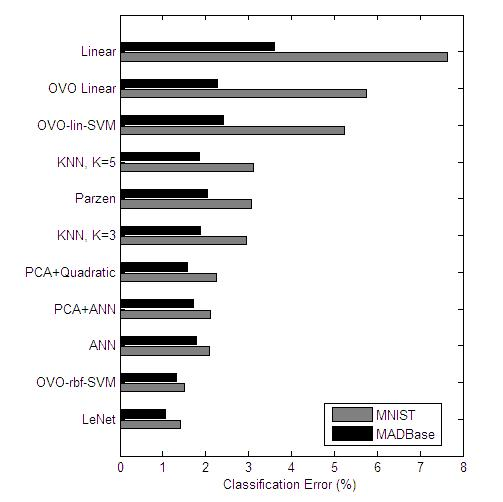
\includegraphics[scale=0.6]{images/fig3.JPG}
      \caption{Comparison of 10 classification techniques on MNIST and MADBase} \label{fig:fig3}
\end{center}
  \end{minipage}
\end{figure*}

Note that the order of arranging the classifiers in Fig.\ref{fig:fig3} is not arbitrary. They are arranged in a descending order form top to bottom according to their classification errors on MNIST. It is clear from Fig.\ref{fig:fig3} that classification errors of different classifiers on MADBase follow the same pattern of decay as the case of MNIST.
The most interesting observation that may be noticed from Fig.\ref{fig:fig3} is that although classification errors of the most powerful classifiers in case of MNIST compared with MADBase, there is a huge gap between classification errors of the weakest classifiers in case of MNIST and their classification error for MADBase.

An explanation for this may be as follows. The Arabic digits recognition problem is in general easier than that of Latin digits. This is why simple classifiers (like linear and OVO linear) score high on MADBase. However, the percentage of the poorly written digits are close for MADBase and MNIST (both around 1\%) and they are equally hard to classify for the weak and the powerful classifiers. See Fig.\ref{fig:fig4} for the patterns misclassified by LeNet for Arabic digits and Fig.\ref{fig:fig5} for Latin digits.
%We believe that there are two reasons.
But why is the Arabic digits recognition problem simpler than that of Latin digits? Two reasons can explain this. The first one is that the interclass distance between each pair of typical (i.e., not poorly written) Latin digits tend to be smaller than that between pairs of Arabic digits. When interclass distance between two digits is small, any variation in writing one digit will lead this digit to be easily confused with the other.

The second reason why Latin digits are harder to classify than Arabic digits is that the variance in writing each of Latin digits is in general higher than that in case of Arabic. In the following two subsections, each of these two proposed reasons is discussed in details.                                   \begin{figure}	
\begin{center}
\subfigure[Latin Digits]{	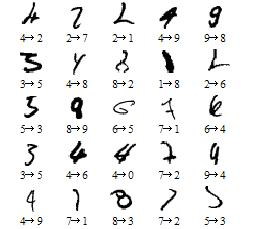
\includegraphics[scale=0.6]{images/hardlatin.JPG} 	\label{fig:fig4}}
\subfigure[Arabic Digits]{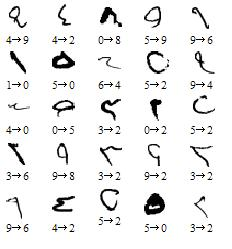
\includegraphics[scale=0.6]{images/hardarabic.JPG} 	\label{fig:fig5}}
	\caption{Samples of hard-to-classify for (a) Latin digits, and for(b) Arabic digits.(misclassified by LeNet)}
\end{center}
\end{figure}                              %                                                            
 \subsection{Interclass distances}
 \label{sec:interclass}%Fig. \ref{fig:fig2}
 \begin{figure*}
\begin{center}
	\centering
		\subfigure[Arabic Digits]{\label{fig:fig6a}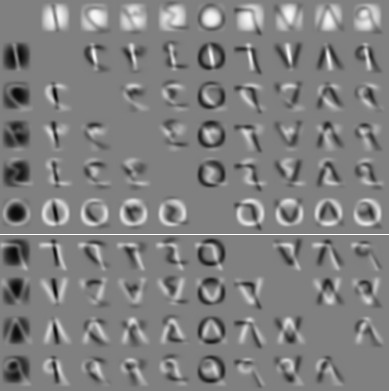
\includegraphics[scale=0.5]{images/fig6arabic.jpg}}
		\hspace{1cm}		
		\subfigure[Latin Digits]{\label{fig:fig6b}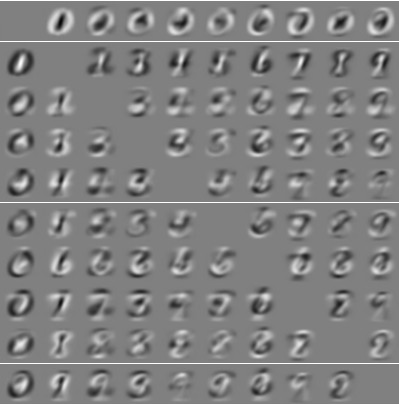
\includegraphics[scale=0.5]{images/figblatin.jpg}}
\begin{center}
	\caption{Image at row $i$ and column $j$ is the result of subtraction digit $j$ from digit $i$ for (a) Arabic digits, and for(b) Latin digits.}\label{fig:fig6}
\end{center}
\end{center}
\end{figure*} 
It is noticed that Latin digits have so many common strokes, and, for many cases, any addition or deletion of a stroke from a Latin digit may lead it to appear as another one. For example, adding a stroke to the upper right of Latin digit '5' will lead it to appear like '9'; and to appear like '6', if a stroke is added at the left bottom of it. Also adding a stroke at the left bottom of '9' leads it to appear like '8'. Digit '4' already appears like '9', and removing the upper stroke of '9' leads it to appear like another writing style of '4'. The fact that Latin digits have many common strokes helps Latin digits to be represented using only 7 strokes in a 7- segment display with natural appearance. But looking at Arabic digits in Table \ref{tab:arabicandlatin}, it is noted that there are not so many common strokes between them, and any attempt to represent them using 7-segment will lead to very artificial appearance (a dot matrix representation is usually used for them in practice). %\ref{fig:fig2},
 
 A visual illustration of this idea is depicted in Fig. \ref{fig:fig6} which shows the resulting images from subtracting the mean of each digit from the means of other digits for both Latin and Arabic digits. The image at row $i$ and column $j$ is the result of subtracting the mean of digit $j$ from that of digit $i$; where foreground (white) is represented by '1' and background (black) is represented by '0'. Each pixel resulting from this subtraction is then added to 1, and then the result is divided by 2. Hence, if the result of subtraction for some pixel location is '-1', it appears as black; if '0', it appears as gray; and if '1', it appears as white. Now, if any two digits have a common stroke, the average of their subtraction will be '0' at the location of this stroke; and hence, will appear gray. Non-common strokes appear black or white depending on which digit is subtracted from the other. It is clear from Fig.\ref{fig:fig6} that Latin digits have many common strokes and hence the gray pixels dominate to the degree that most of the digit pairs are not distinguishable from each other. On the other hand, for Arabic digits, most of digit pairs are quite distinguishable.
\begin{figure}
	\centering
		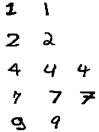
\includegraphics[scale=0.7]{images/fig7.JPG}
	\caption{ Some Latin digits and their different typical writing styles.}
	\label{fig:fig7}
\end{figure}
%Fig. 7. Some Latin digits and their different typical writing styles.
The above is rather an informal evidence. In the following,a more formal numerical evidence is going to be introduced. A numerical measure for the interclass distance between a pair of classes $(i,j)$, i.e. between digit $i$ and digit $j$, may be the Euclidean distance $d_{ij}$ between their means,
\[
{\rm  }d_{ij}  = \sqrt {\sum\limits_{\forall x} {\sum\limits_{\forall y} {\left[ {\mu _i (x,y) - \mu _j (x,y} \right]^2 } } } 
\]
where, $i,j= 0,1,,9$; $x,y = 1,2,,28$; and $\mu _i (x,y)$ is the mean value of the pixel at location $(x,y)$ of the images of digit $k$,
\[
\mu _k (x,y) = \frac{1}{N}\sum\limits_{n = 1}^{N_k } {I_{kn} (x,y)} 
\]
where $I_{kn}(x,y)$ is the pixel value at location $(x,y)$ of the $n^{th}$ image of the training set of digit $k$, and $N$ is the number of training samples of digit $k$.
A numerical measure for the overall separation between all class pairs ($d_{overall}$) may be the summation of $d_{ij}$ for all $i$ and $j$, i.e., 
\[
{\rm d}_{{\rm overall}}  = \sum\limits_{\forall i} {\sum\limits_{\forall j} {d_{ij} } } 
\]
The value of $d_{overall}$ was found for Arabic digits to be larger than that of Latin by 11.9\%. This means that interclass separations between Arabic digits are larger than that in case of Latin. To check the significance of this result, the hypothesis of having the $d_{overall}$ equal for both cases Latin and Arabic is checked. To do so, the training set is partitioned into 6 separate subsets, each containing 10,000 samples. The $d_{overall}$ measurement is calculated for each subset resulting in 6 different measurements. This is done for both cases Latin and Arabic. A t-test \cite{MathBook25} is then performed to check the hypothesis that Latin and Arabic have equal mean value of $d_{overall}$. The hypothesis was found to have a p-value of $4.3 \times 10^{ - 8} $, which means that it can be rejected with very small significance level.
\subsection {Variances}
The second reason why Latin digit recognition problem is harder than that of Arabic is that variances in writing Latin digits are larger than that of Arabic. One measure of variances (scattering) $S_k$ of some pattern $k$ around its mean is the trace of its covariance matrix ~\cite{PatternBook10}, 
\[
S_k  = tr\left[ {\sum\nolimits_k {}  } \right] = \sum\limits_{i = 1}^d {\sigma _{ki}^2 } ,
\]
,where $\sum\nolimits_k {}$is the covariance matrix of pattern $k$, $\sigma _{ki}^2$ is the variance of the $i^{th}$ dimension of pattern $k$, and $d$ is the dimensionality of the pattern. For digit recognition problem, the scattering of some digit $k$ around its mean is then given by,
\[
S_k  = \frac{1}{{N_k }}\sum\limits_{n - 1}^{N_k } {\sum\limits_{\forall x} {\sum\limits_{\forall y} {\left[ {I_{kn} (x,y) - \mu _k (x,y)} \right]^2 } } } 
\]
A numerical measure for the overall scattering is $S_{overall}  = \sum\limits_{k = 0}^9 {S_k }$. It is found that $S_{overall}$ for Latin digits is 27.9\% larger than that of Arabic. This means that large deviation from the mean is more probable for Latin digits than that for Arabic. The reason behind this might be the fact that Latin digits have many writing styles as shown in Fig. \ref{fig:fig7}.	

To check the significance of the $S_{overall}$ comparison between Arabic and Latin digits, the training set is partitioned into 6 separate subsets, each containing 10,000 samples. The $S_{overall}$  measurement is calculated for each subset resulting in 6 different measurements. This is done for both cases Latin and Arabic. A t-test~\cite{MathBook25} is then performed to check the hypothesis that Latin and Arabic have equal mean value of $S_{overall}$. The hypothesis was found to have a p-value of $1.1\times10^{-11}$. This means that the hypothesis can be rejected with very small significance level.
\section {Conclusion} %{CONCLUSION}
\label{sec:conclusion}
A comparison between the performances of 10 classifiers is made on both Arabic and Latin handwritten digit recognition problems. An interesting result of such comparison is that while the performances of the most 
powerful classifiers on Arabic and on Latin digits are close, the weaker classifiers show very good performance on Arabic digits unlike their performance on Latin digits. The reason behind this is suggested to be that Arabic handwritten digits recognition problem is in general easier than that of its Latin counterpart. An analysis is given for the reasons why Arabic digits are in general easier to classify than Latin digits and it has been found that this is because interclass distances between Arabic digits are larger than those of Latin and variances in writing Arabic digits are smaller.

The practical implications of the findings of the comparison presented in this paper  become evident in the case of the Arabic handwritten digits recognition problem in applications where classification speed is a concern. In those applications, weaker classifiers may present a plausible alternative to powerful ones. In classification cascades for example, weaker yet faster classifiers play prominent role at the early stages of the cascade to speed up the performance of the whole cascade~\cite{optimumPaper,GreedyPaper} It is expected that weaker classifiers play a more significant role in Arabic handwritten digits classification cascades than their role in the Latin case due to their superior performance in Arabic digits classification.

% \section {Acknowledgment}%{ACKNOWLEDGMENT}
%This research is supported by a grant from the American University in Cairo (AUC). 
\bibliographystyle{unsrt}
%\bibliographystyle{latex8}
\bibliography{../../library}
\end{document}
